\chapter{Predizione della struttura di proteine (PSP)}

Il protein folding problem ha sia guidato che tratto beneficio dagli avanzamenti nei metodi sperimentali e computazionali\supercite{dill2008protein}. Uno dei maggiori obiettivi della biologia computazionale è proprio il PSP (Protein Structure Prediction), ovvero la predizione della struttura nativa tridimensionale di una proteina a partire dalla sua sequenza amminoacidica. Il PSP è il problema opposto al \textit{protein design} (la progettazione di nuove sequenze proteiche aventi delle specifiche attività).

\par Grazie al CASP\footnote{Critical Assessment of Structure Predictions, vedi la sezione \ref{sec:CASP}.}, alla crescita del PDB, ai metodi per omologia e di allineamento di sequenze, i metodi computazionali hanno registrato incredibili progressi, come dimostra il livello raggiunto da AlphaFold. 

\par La predizione della struttura di proteine è uno strumento fondamentale: in medicina per la comprensione delle malattie da misfolding, nell'industria farmaceutica per risparmiare anni di laboriosi e costosi esperimenti correntemente richiesti per lo sviluppo di un singolo farmaco (\textit{drug design}), in biotecnologia per il design di nuovi enzimi e in generale per acquisire maggior conoscenza sul protein folding in tutti i suoi lati.

\section{Metodi e strumenti informatici}
La piccola percentuale di strutture determinate e il gap che continua a crescere con le sequenze conosciute (vedi sotto la sezione \ref{sec:database}) è una conseguenza della lentezza e della dispendiosità dei metodi sperimentali (e in parte anche dei progressi delle tecnologie di sequenziamento). I metodi computazionali, significativamente più veloci ed economici, potrebbero fornire una possibile soluzione a questo problema.

\subsection{Workflow e classificazione dei metodi per il PSP}
%kessel 3.4 [computational methods for structure prediction]
%pal 15.3.2 Computational structure prediction. Molto breve
%pal 18.1 [molecular dynamics]
%psp-wiki [abbastanza discorsivo]
%prot-eng-wiki[molto breve]
%Gu 28-33 [serie di articoli messi insieme, sembra stra interessante]
%baxevanis 12 p.385 \\ \\

Quando si parla di metodi per la predizione della struttura di proteine esistono due \textit{paradigmi fondamentali} per affrontare il problema:
\begin{itemize}
	\item paradigma \textit{ab initio}
	\item paradigma \textit{data-based}
\end{itemize}

Il paradigma \textit{ab initio} (o \textit{de novo}) si basa su un approccio puramente fisico, nel quale la struttura è predetta da zero simulando principi fisici.

\par Nel paradigma \textit{data-based} invece si fa uso di informazioni estratte da database di sequenze o strutture di proteine. I metodi basati su questo paradigma sono dominanti nei metodi odierni. Tale maggioranza è legata alla crescita notevole della quantità di dati disponibili. È importante notare che i \textit{paradigmi} fanno riferimento al modo in cui si affronta il problema, alla direzione dalla quale si prova a risolverlo.

\par Le proteine che esistono in natura oggi si sono sviluppate attraverso lunghi processi evoluzionistici, progredendo attraverso mutazioni casuali e selezione naturale. La rivoluzione genetica degli anni '50, consentendo la determinazione delle sequenze amminoacidiche, ha permesso il nascere di metodi di confronto delle sequenze. È per questo che si possono ricavare informazioni sulla struttura 3D di una sequenza amminoacidica cercando altre proteine con proprietà nella sequenza simili e una struttura nota. Se si trova una similitudine globale si parlerà di \textit{template}. È da qui che nasce la famosa distinzione fra \textit{template-based modeling} (TBM) e \textit{template-free modeling} (FM). 

\par Come già accennato, nel panorama attuale quasi tutti gli approcci oggi utilizzati per il PSP sono prevalentemente \textit{data-based}: i metodi puri \textit{ab initio} vengono raramente utilizzati per la predizione della struttura di proteine (per ragioni che verranno spiegate in dettaglio nella sezione \ref{sec:ab-initio}). Tuttavia, nella pratica, alcune intuizioni del paradigma \textit{ab initio} vengono usate in metodi \textit{data-based}, ad esempio la funzione euristica di valutazione che simula il campo di forza per calcolare l'energia potenziale.

\par È possibile dividere i metodi \textit{data-based} sviluppati in due grandi categorie, a seconda della loro funzione:
\begin{itemize}
	\item manipolazione della sequenza di input
	\item modellazione della struttura della proteina target
\end{itemize}

Nella prima categoria vi sono i metodi di MSA (\textit{Multiple Sequence Alignment}), \textit{fold recognition} e \textit{contact prediction}. Nella seconda categoria invece si trovano i metodi di \textit{homology modeling}, \textit{threading}, \textit{fragment-based} e i metodi di modellazione di regioni non allineate (\textit{loop-modeling} e \textit{side-chain modeling}).

\begin{figure}[!htb]
	\centering
	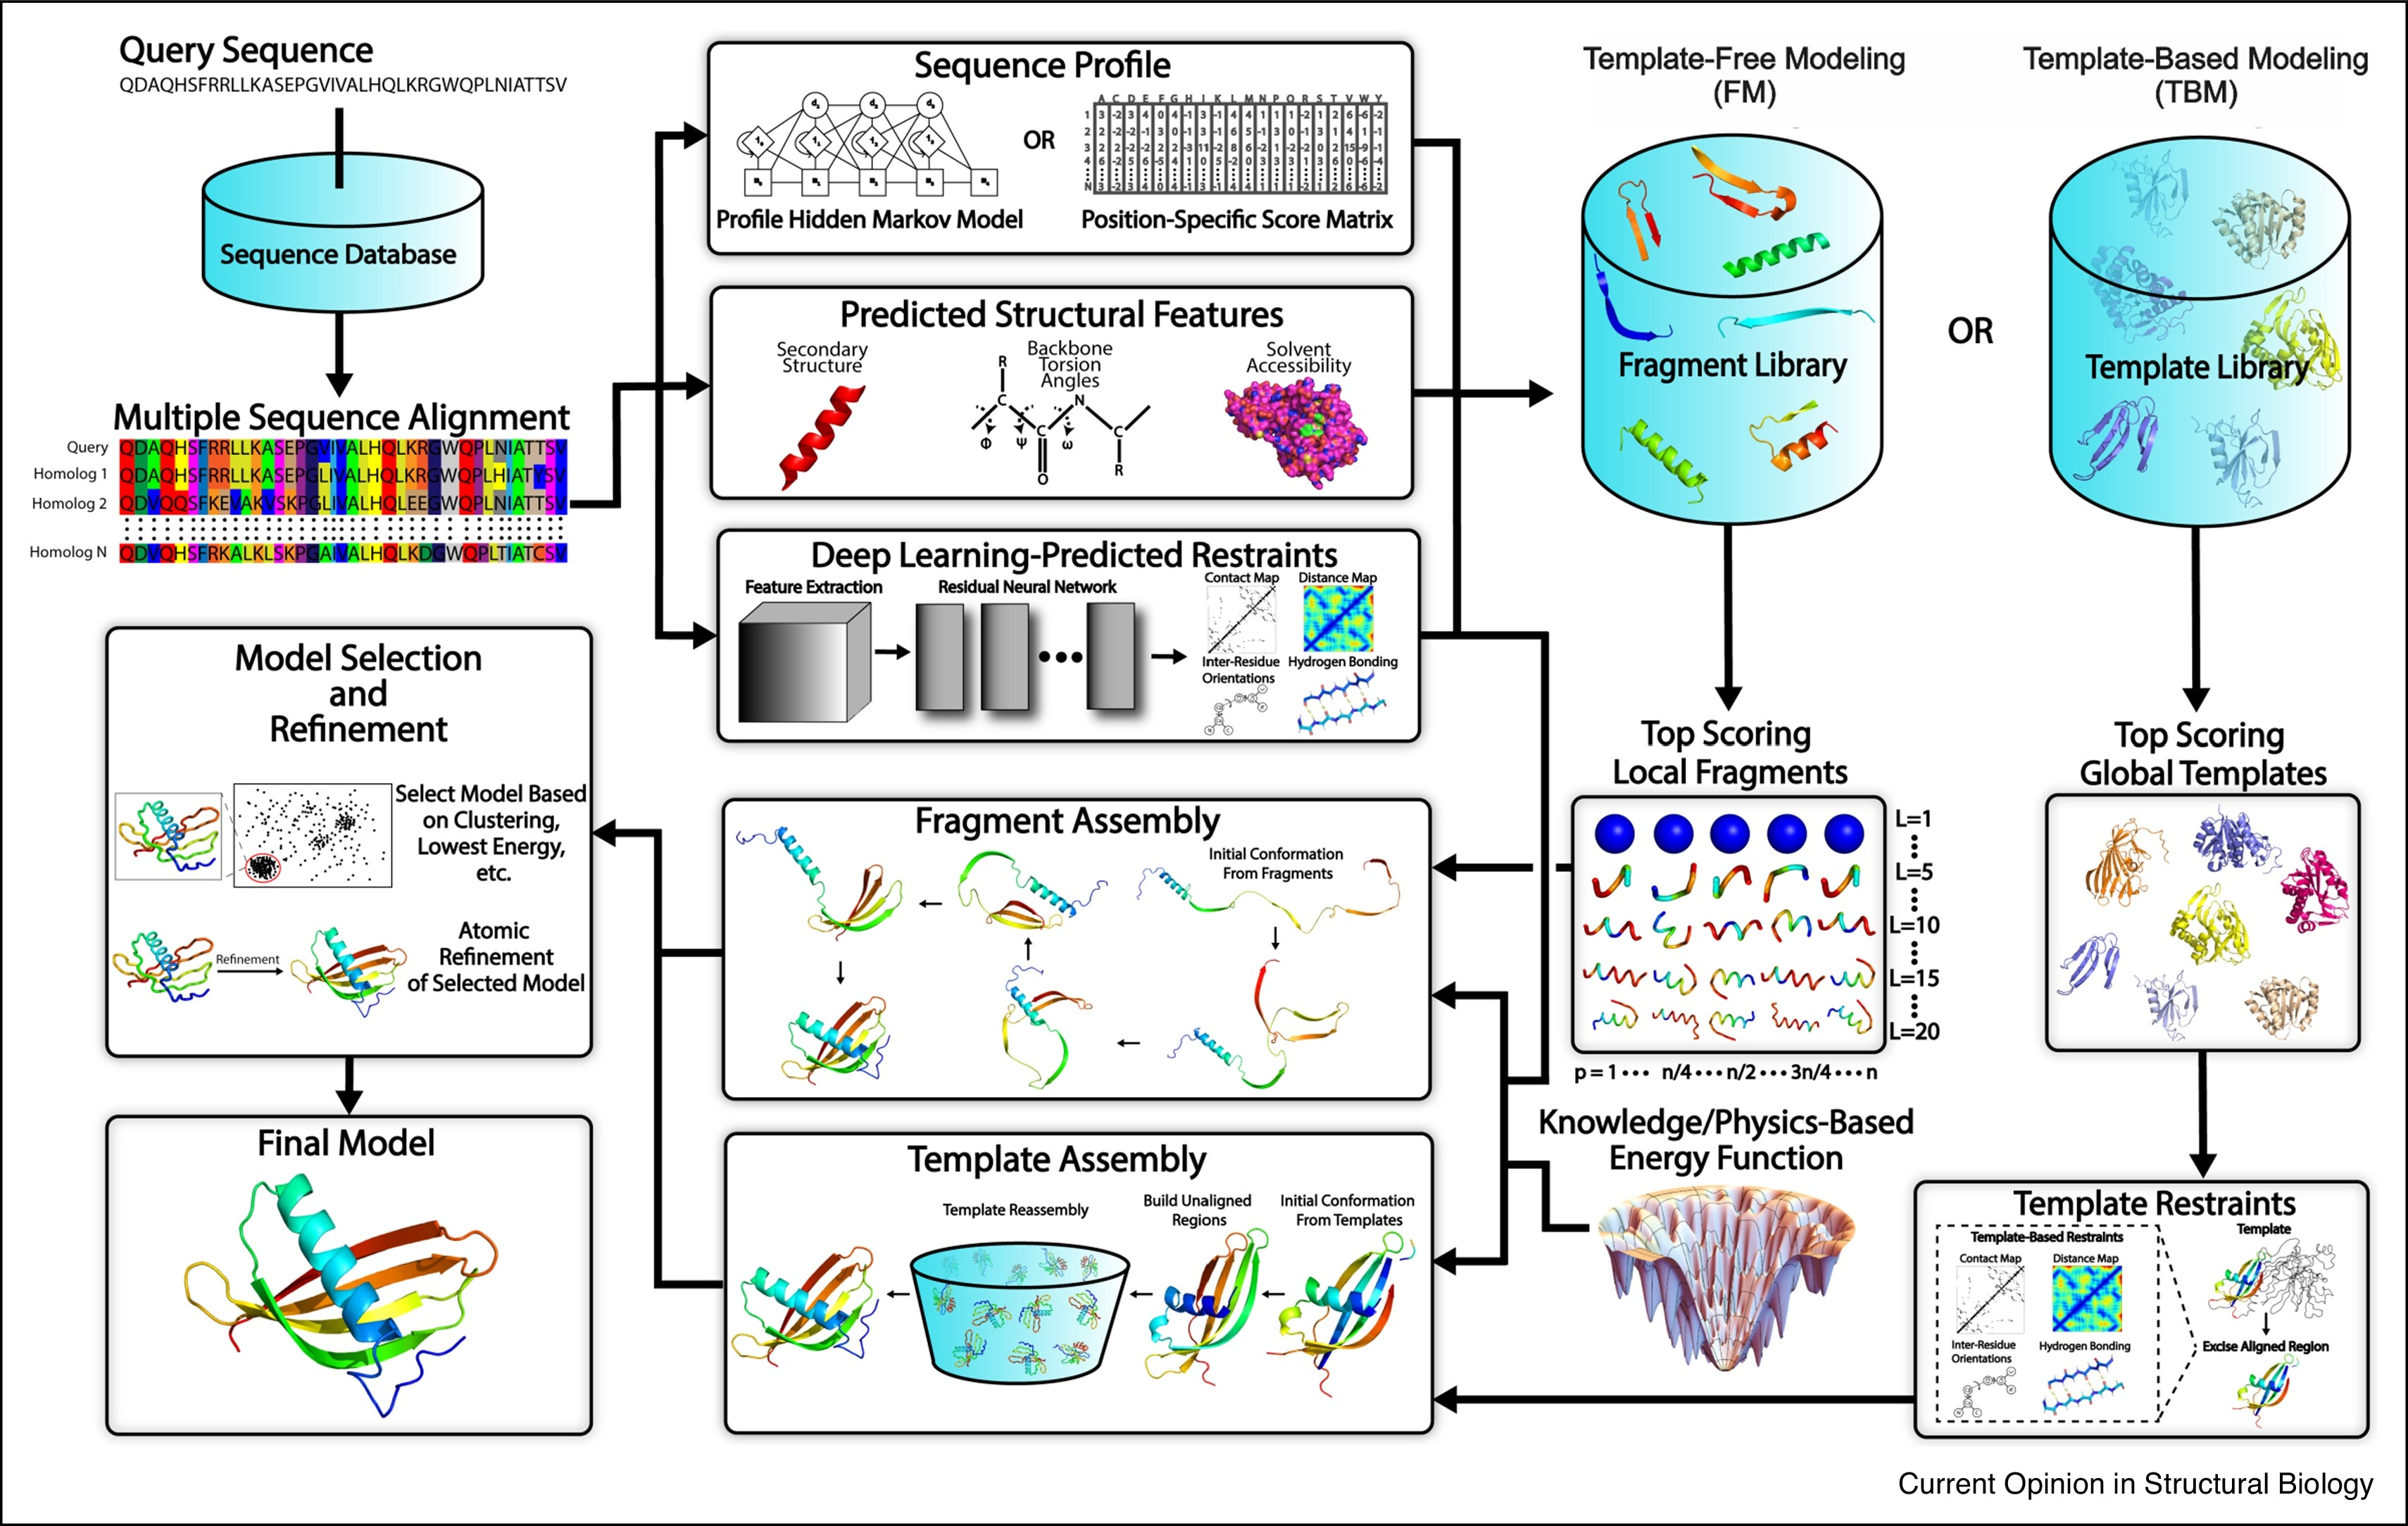
\includegraphics[scale=0.95]{images/FM-TBM.jpg}
	\caption{Step tipici negli approcci al PSP di tipo TBM e FM. Fonte\cite{pearce2021deep}}
	\label{fig:fm-tbm}
\end{figure}

\par  Quando si ha di fronte una sequenza di una proteina senza struttura nota e si vuole predire la sua forma tridimensionale, un metodo per il PSP attuale agirebbe nel seguente modo (vedi fig. \ref{fig:fm-tbm})\footnote{Tutto ciò che viene citato verrà spiegato nel dettaglio successivamente, viene ora riportato con l'obiettivo di fornire una visione globale degli argomenti.}:
\begin{enumerate}
	\item viene generata una MSA per identificare sequenze omologhe a partire dalla sequenza della proteina
	\item l'MSA viene poi convertita e profilata; vengono predette caratteristiche strutturali (come strutture secondarie o esposizione al solvente) e i contatti fra i residui
	\item viene scelto il tipo di modellazione adeguato
	\item vengono assemblati i frammenti o i template
	\item viene scelto il modello fra vari candidati, che sarà poi raffinato a livello atomico
\end{enumerate}

\par Nel 1° passo l'obiettivo è identificare sequenze omologhe. Se si riesce a trovarne almeno una allora è possibile procedere alla \textit{modellazione per omologia} (\textit{homology modeling}). \\

\par Nel 2° passo si applicano dei protocolli di \textit{fold recognition} al fine di ricavare informazioni strutturali per due scopi:
\begin{itemize}
	\item identificare altri template globali al fine di applicare protocolli di \textit{threading} 
	\item se non se ne trovano, tali informazioni verranno utilizzate per valutare i frammenti nella ricerca all'interno di una \textit{fragment library}
\end{itemize}

Vengono anche predetti i contatti fra residui sulla base di informazioni co-evolutive (\textit{correlated mutation}), generando o una \textit{contact map}, o un \textit{distrogramma} o una \textit{distance map} attraverso una \textit{deep residual neural network} (\textit{ResNet}). Il fine è ricavare restrizioni spaziali come contatti inter-residuo a lunga distanza, distanze specifiche, legami idrogeno e angoli di torsione. \\

\par Si rientrerà nel caso del TBM sia che venga eseguita una modellazione per \textit{omologia} che una modellazione basata sul \textit{threading}.
Si rientra invece nel caso del MF quando non si riescono a trovare dei template globali. In questo caso vengono principalmente utilizzate tecniche di modellazione \textit{fragment-based}, ovvero basate su frammenti di proteine che verranno poi integrati. Nel 3° passo, a seconda che ci si trovi nel caso TBM o MF vengono attuate le rispettive modellazioni.\\ 

\par Nel 4° passo l'assemblaggio è eseguito sotto la guida di una funzione euristica del campo di forza, che può essere \textit{energy-based} e/o \textit{knowledge-based}, combinata con una rete neurale profonda per la predizione di determinate caratteristiche. Nel caso di una modellazione TBM si hanno delle restrizioni spaziali sul modello. Vengono utilizzate tecniche specifiche per regioni non allineate, come i loop (\textit{loop modeling}). \\

\par Nel 5° passo vengono valutati i modelli, viene eseguita una valutazione della qualità (\textit{quality assessment, QA}) stimando l'accuratezza del modello (\textit{estimation of model accuracy}, \textit{EMA}) e infine viene eseguito il raffinamento. Tipicamente viene scelto il modello con minore energia. \\

\par Come si può notare, l'approccio maggiormente usato in questo \textit{workflow} è quello \textit{data-based}. Vengono utilizzate in combinazione varie tecniche: non vi è una singola tecnica principale.

\subsubsection{Nota sulla classificazione dei metodi}

La predizione della struttura di proteine è stato ed è tutt'ora un campo in evoluzione. Per tale ragione risulta difficile classificare e raggruppare i metodi in nette categorie. Il CASP divide i metodi in due classi principali: TBM  e FM\supercite{abbass2020enhancing}, in base all'utilizzo o meno di informazioni prese da template (proteine con struttura 3D nota). 

\par Nonostante questa divisione possa risultare efficace, in questo lavoro si è ritenuto opportuno non seguire una classificazione standard e provare a delineare invece le idee alla base degli approcci e raggrupparli in più livelli secondo questo principio. La motivazione risiede nel fatto che nessun metodo preso singolarmente può dare risultati soddisfacenti: negli anni si è assistito infatti ad un utilizzo combinato dei tanti metodi trovati (come la figura \ref{fig:fm-tbm} e la sezione sopra può mostrare) sfocando sempre più i margini fra le categorie. Tutto questo ha creato confusione ed un utilizzo improprio dei termini. Come si vedrà, \textit{ab initio} indica il "puro" approccio fisico, mentre con la divisione operata dal CASP si tende spesso ad utilizzare come sinonimi \textit{ab initio} e \textit{template-free} methods, cosa che, in fase di stesura della tesi, è stata reputata equivoca e forse erronea. Allo stesso tempo i metodi si sono evoluti negli ultimi anni, specialmente con l'avvento del Deep Learning, e le vecchie classificazioni \footnote{Compresa quella di \fullcite{kessel_ben-tal_2018}. Nonostante ciò il presente capitolo si basa in parte sul capitolo 3.4 del libro appena citato.} non rispecchiano più l'attuale struttura dei metodi usati. Si è deciso di focalizzare l'attenzione sulla struttura dei metodi per il PSP odierni e da qui provare ad astrarre verso l'alto per classificare i vari approcci possibili in 2 categorie funzionali e infine in due grandi paradigmi. Il quadro di riferimento è il \textit{workflow} della figura \ref{fig:fm-tbm}, che delinea la struttura tipica degli approcci TBM ed FM attuali. 

\subsection{L'arrivo del Deep Learning}

avanzamenti nel PSP grazie al DL:
advances in MSA generation, contact map prediction, protein
residue–distance prediction, potentials to guide iterative fragment assembly, models, or
quality assessment (QA), advances in overall protein prediction pipelines, and advances
in Cryo-EM based protein structure determination and the future outlook for the protein
structure prediction field.


\subsubsection{Paradigmi nel soft computing}
% \subsubsection{ANN, EC, SVM, .. [..]}


\subsection{Database e rappresentazione delle informazioni} \label{sec:database}
% pal 6.4.1 p.145
% Gu 10-13 p.468
% baxevanis 12 p.367

Come si è già visto è possibile descrivere una proteina attraverso la sua sequenza amminoacidica. Il risultato è una stringa di lettere alfabetiche, poiché ogni amminoacido corrisponde ad una determinata lettera (vedi fig. \ref{fig:codici-amminoacidi}). Si ricorda anche che ad un amminoacido può corrispondere uno o più codoni (3 paia di basi azotate nel DNA). \\

\par Per quanto riguarda la struttura delle proteine, il formato standard è il PDB (Protein Data Bank).

\subsubsection{Database di proteine}



--PDB--
The Protein Data Bank (PDB) is an archive of experimentally determined three-dimensional
structures of biological macromolecules that serves a global community of researchers, educators,
and students. The data contained in the archive include atomic coordinates, crystallographic
structure factors and NMR experimental data. Aside from coordinates, each deposition also
includes the names of molecules, primary and secondary structure information, sequence
database references, where appropriate, and ligand and biological assembly information, details
about data collection and structure solution, and bibliographic citations.


\par La predizione della struttura è importante per un semplice motivo: i biochimici conoscono oggi la sequenza amminoacidica per più di 225 milioni di proteine\supercite{proteienDBentries} (UniProt, con circa 4.5-5 milioni aggiunte ogni mese) ma sono state determinate solamente circa 160.000 strutture tridimensionali di proteine\supercite{proteienDBentries} (PDB\footnote{Al 3 Febbraio 2022 sono presenti 162.913 strutture di proteine nella versione dell'RCSB. Nel PDB ci sono anche strutture di altre macromolecole (complessi di acidi proteici-nucleici, DNA e RNA) per un totale, incluse le proteine, di 186670\supercite{pdbStats}. Nel wwPDB (database globale) vi sono in totale 197961 strutture di macromolecole\supercite{wwpdbStats}.}, con poco più di 10.000 strutture aggiunte ogni anno). 

\begin{figure}[!htb]
	\centering
	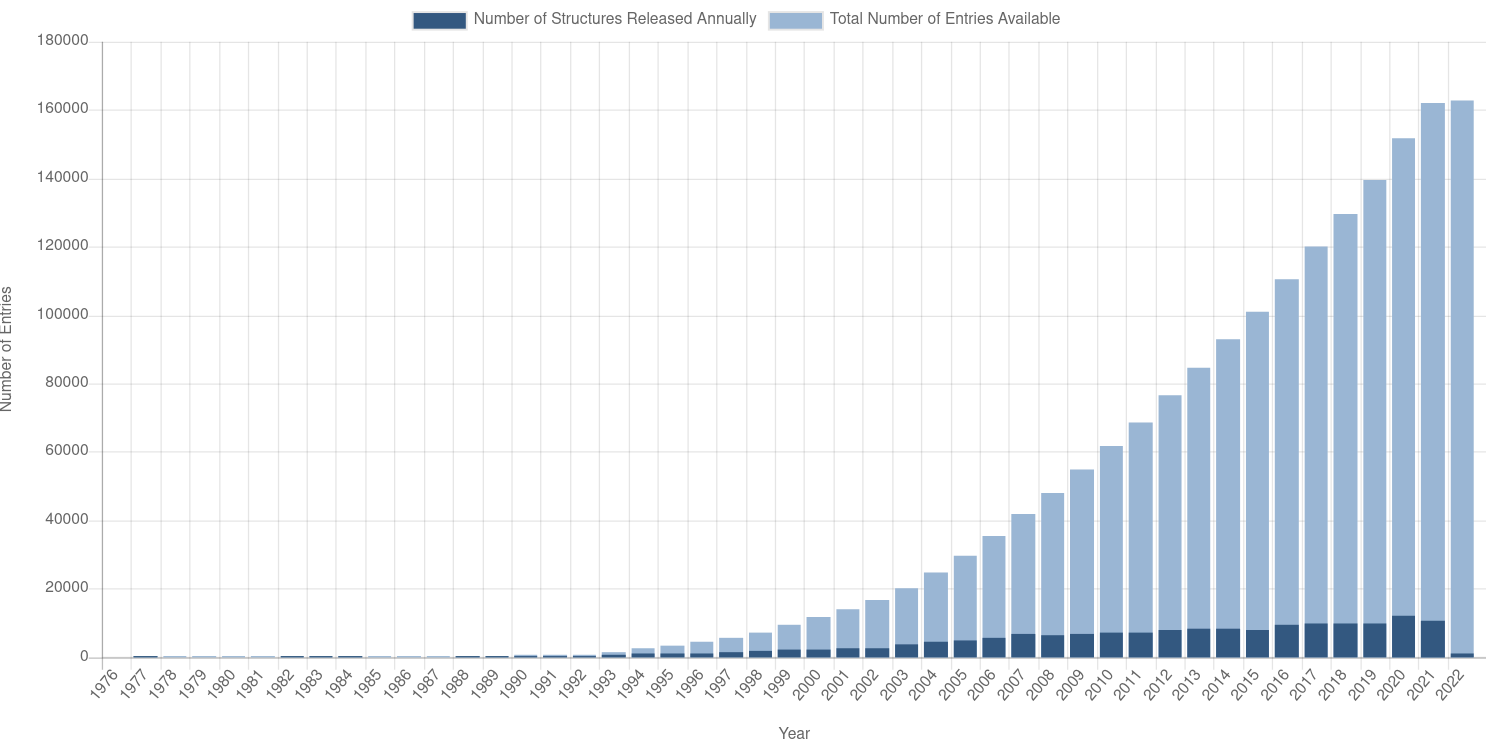
\includegraphics[scale=0.3]{images/pdb-statistica.png}
	\caption{Crescita complessiva del numero di strutture di proteine pubblicate nel PDB. Fonte\cite{pdbStats}}
	\label{fig:pdb-statistica}
\end{figure}


%baxevanis 12 p.373, 1





\subsection{Rappresentazione grafica}
%pal 6.4 p.146, ottima
%kessel p.174 (2.3 GRAPHIC REPRESENTATIONS OF PROTEINS)

\subsection{CASP}
%-abbass 2020
Dal 1994 il campo del PSP è stato stimolato, monitorato e quantitativamente valutato dalla competizione biennale CASP (\textit{Critical Assessment of Structure Predictions}). CASP è una sfida nella quale gruppi di ricerca si sfidano cercando di realizzare predizioni di strutture di proteine. È nota la sequenza amminoacidica di queste proteine target ma non la struttura sperimentale. Queste sequenze di proteine provengono da laboratori sperimentali congiunti: è pianificata la determinazione delle loro strutture native in vitro, che verrà infine utilizzata per stabilire l'accuratezza dei metodi in gara.

\par Questi esperimenti a livello di comunità sono cresciuti significativamente nel corso delle edizioni: dai 33 target e i 100 modelli sottomessi nel 1994 (CASP1) agli 82 target e più di 55.000 modelli sottomessi nel 2018 (CASP13)\supercite{abbass2020enhancing}.

\par Ogni due anni un insieme di sequenze di proteine sono rilasciate gradualmente nel corso di un paio di mesi, durante i quali gruppi di ricerca da tutto il mondo tentano di predire le loro strutture 3D e inviano i loro modelli (fino a 5 per target).

\par Nei primi 6 round (CASP1-6), i target erano classificati in 3 categorie: \textit{comparative modeling}, \textit{fold recognition} e \textit{ab initio}. Da allora i target sono stati classificati solo in 2 classi: le famose \textit{template-based modeling} e \textit{template-free modeling}. I target nella categoria TBM sono considerati "facili" mentre quelli in FM sono considerati difficili. È presenta anche la divisione fra metodi completamente automatici e previsioni ottenute usando intervento umano.

\par I risultati sono valutati sulla base di vari criteri, come il numero di residui la cui posizione è stata predetta con un certo livello di accuratezza, identificazione di strutture secondarie, limiti dei domini, contatti fra residui, regioni disordinate, ecc.

\par Analizzando i risultati del CASP negli anni si può notare che i metodi basati su un approccio fisico, nonostante l'aumento della potenza computazionale, hanno subito solo lievi miglioramenti.

\par L'importanza del CASP per la biologia strutturale è alta anche per il contributo che ha dato alla creazione dei metodi automatici, accessibili anche ai non esperti.

\par Nel 2020 gli organizzatori del CASP14 hanno riconosciuto AlphaFold come soluzione del \textit{protein–structure–prediction problem} ???. \\


%\subsection{Input, output, valutazione}
%\subsubsection{Proprietà dei dati di input}

\subsubsection{Output: modelli, ... [..]}
\subsubsection{Metriche di valutazione}
%- Gu 16 p.655 GENERAL APPROACH TO STRUCTURE COMPARISON AND ALIGNMENT
%baxevanis 12 p.386



\section{Paradigma \textit{ab initio}} \label{sec:ab-initio}
{
Il metodo più lineare e a prima vista ovvio per predire la struttura nativa di proteine è seguire la natura, simulando accuratamente come le forze fisiche guidino la proteina a ripiegarsi e usare questa simulazione per riprodurre il processo di ripiegamento su proteine con strutture sconosciute. \textit{Ab initio}, termine latino, significa infatti "dall'inizio". Questo approccio si basa sul postulato di Anfinsen.

\par Il primo problema che sorge è superare il paradosso di Levinthal. Per farlo si assume un profilo energetico a imbuto del ripiegamento, ovvero la premessa termodinamica che la forma nativa di una proteina sia lo stato in cui risulta avere più bassa energia libera, o più precisamente (richiamando la definizione di struttura nativa data nella sez. \ref{sec:energetica}) quella conformazione avente minore energia libera tale da mantenere il livello di dinamicità richiesto alla proteina per svolgere la sua funzione biologica.

\par Le predizioni nell'approccio \textit{ab initio} sono pertanto \textit{energy-based}, ovvero guidate dall'idea di minimizzare l'energia. Si può vedere il PSP secondo l'approccio \textit{ab initio} come un problema di ottimizzazione dove una funzione di energia gioca il ruolo di \textit{euristica} cercando di raggiungere il minimo globale di energia all'interno dello spazio di ricerca. In quanto \textit{energy-based} usano solo informazioni sul tipo di atomi nel sistema, le loro posizioni relative nello spazio tridimensionale e le loro interazioni con gli altri atomi. Viene poi calcolato l'intero contenuto di energia del sistema e le forze agenti su ogni atomo. 

\par L'energia totale di un sistema (\textit{free energy}) può essere decomposta in varie componenti: cinetica, potenziale, termica ecc. È l'energia libera che determina la stabilità del sistema. Come si vedrà sotto, nell'approccio fisico non viene calcolata tutta l'energia libera ma viene approssimata con una sua parte per motivi di complessità.

\par Sebbene vi siano differenti metodi in questo approccio, tutti condividono due caratteristiche di base:
\begin{itemize}
	\item calcolano il contenuto di energia del sistema in una singola configurazione
	\item campionano numerose configurazioni e ne trovano una con la minor energia libera
\end{itemize}

Per \textit{configurazione} si intende la disposizione complessiva di tutti gli atomi di tutti i componenti del sistema (proteina, solvente, ioni, membrana ecc.) mentre la posizione collettiva dei soli atomi della proteina viene chiamata \textit{conformazione}.

\subsubsection{Molecular mechanics \& dynamics}

\par Per descrivere in maniera affidabile tutte le forze fisiche operanti sul sistema tra i differenti atomi bisognerebbe descriverne la distribuzione di tutti gli elettroni, il che richiede però calcoli di meccanica quantistica (QM). Le forze, in un sistema molecolare, risultano dalla distribuzione spaziale degli elettroni attorno agli atomi. Sfortunatamente questi calcoli sono computazionalmente molto costosi e una rigorosa caratterizzazione di un sistema macromolecolare, con milioni di atomi, è al momento insostenibile. Calcoli di QM su una singola conformazione di una piccola proteina possono richiedere mesi, tempi troppo lunghi se si ha l'obiettivo di provare tante configurazioni per sceglierne una finale. 

\subsubsection{Molecular mechanics}

\par Per le ragioni sopra elencate gli scienziati spesso investigano sistemi macromolecolari usando approssimazioni delle reali forze in essi. Il campo da cui i calcoli per le approssimazioni sono presi è chiamato \textit{molecular mechanics} (MM), poiché approssima sistemi molecolari usando espressioni prese dalla meccanica newtoniana classica:
\begin{itemize}
	\item il contenuto di energia è descritto usando un \textit{campo di forza} nel quale gli atomi e i legami covalenti sono trattati come palline e molle
	\item le descrizioni che richiederebbero calcoli di QM vengono ignorate
	\item le rappresentazioni sono \textit{esplicite}: prendono in considerazione tutti gli atomi (vedi fig. \ref{fig:descrizione-esplicita-mm})
\end{itemize}

Il campo di forza sopra accennato descrive l'energia potenziale del sistema. Da notare che l'energia potenziale (intesa come entalpia) è solo una delle due componenti dell'energia libera, vedi sez. \ref{sec:energetica}).

\par Un campo di forza è un'energia di posizione: l'energia di un oggetto in una specifica posizione all'interno di un campo (gravitazionale, elettrico, magnetico ecc.). Nelle molecole l'energia potenziale è la somma di tutti gli effetti dei campi elettrici atomici\footnote{gli atomi possiedono, in base alla loro eventuale carica, campi elettrici che influenzano gli altri atomi} in una determinata posizione. Si può approssimare l'energia potenziale all'energia risultante da tutti i legami covalenti e le interazioni non covalenti, escluse quelle non polari \footnote{Un esempio di interazione non polare è l'effetto idrofobico. Vengono escluse poiché coinvolgono principalmente cambiamenti di entropia nel solvente.}, in una singola configurazione del sistema. In genere i campi di forza non sono una singola funzione ma una somma di più termini, ognuno corrispondente a un differente tipo di legame chimico o interazione, un esempio:

\[ U_{tot}=U_{cov}+U_{elst}+U_{vdw} \]

dove per $U_{tot}$ si intende l'energia potenziale totale, per $U_{cov}$ l'energia potenziale dei legami covalenti, per $U_{elst}$ quella delle interazioni elettrostatiche e per $U_{vdw}$ quella delle interazioni di van der Waals.

\par L'energia potenziale delle interazioni elettrostatiche può essere calcolata con la legge di Coulomb, mentre quella delle interazioni di van der Waals tramite l'equazione di Lennard-Jones. Nelle simulazioni di sistemi biologici vengono usati: CHARMM, AMBER, GROMACS, ecc.

\begin{figure}[!htb]
	\centering
	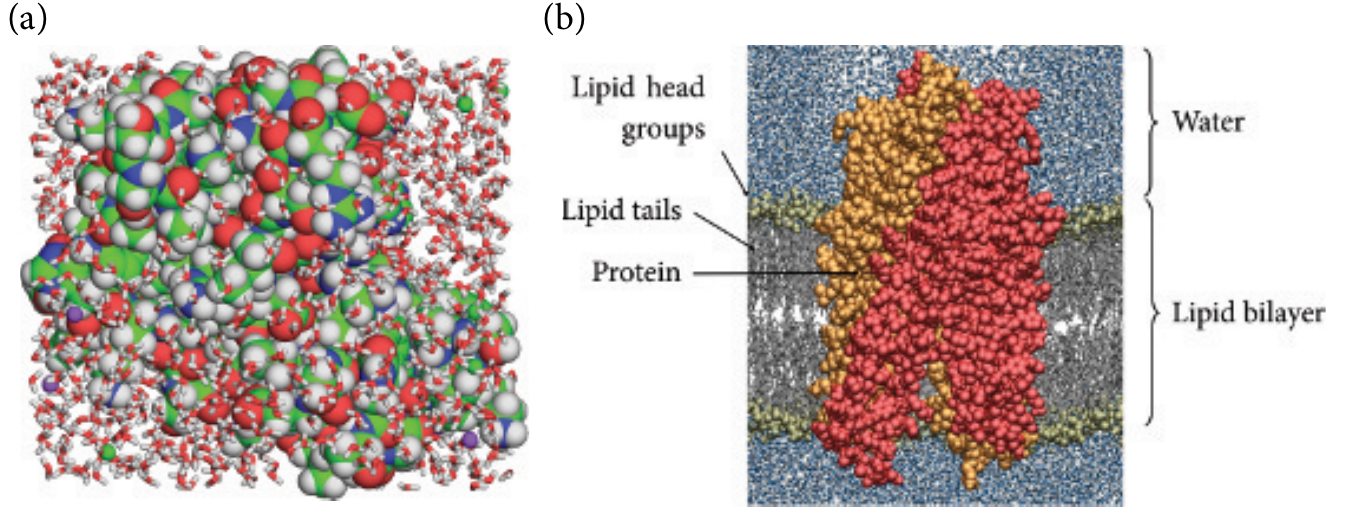
\includegraphics[scale=0.4]{images/esplicita-mm.png}
	\caption{Descrizioni esplicite nei calcoli di MM. (A) una piccola proteina immersa in un solvente composto da molecole d'acqua e ioni (Na$^{+}$, Cl$^{-}$). La proteina è rappresentata come sfere di atomi, l'acqua come bastoncini e gli ioni come piccole sfere magenta e gialle. (B) una proteina trasportatrice in un doppio strato lipidico, circondato da ambiente acquoso. La proteina e le teste dei lipidi sono rappresentate in modo space-fill, mentre l'acqua e le code dei lipidi con rappresentazione wire-frame. Fonte \cite{kessel_ben-tal_2018}}
	\label{fig:descrizione-esplicita-mm}
\end{figure}

\par La descrizione approssimata fornita dal campo di forza permette di calcolare l'energia potenziale di molti sistemi macromolecolari in meno di un secondo. \\

\par Una variante del MM è la \textit{QM/MM} nella quale i calcoli di QM sono indirizzati solamente su una piccola parte della proteina che contiene residui funzionali importanti. Le altre regioni sono soggette invece a MM, con calcoli molto più veloci \footnote{questo approccio è stato introdotto da Warshel, Levitt e Karplus}

\subsubsection{Spazio configurazionale}

\par Assumendo l'accuratezza del campo di forza, il calcolo dell'energia potenziale di un sistema consente di determinare (parte del)la stabilità di una configurazione. L'idea iniziale potrebbe essere quella di considerare tutte le possibili locazioni atomiche del sistema, calcolare l'energia potenziale in ogni caso e scegliere quella con la minor energia. Come si può facilmente intuire ciò risulta essere un procedimento troppo oneroso, in quanto si devono considerare anche gli atomi del solvente (ed eventuali ligandi o cofattori). Anche il solo numero delle possibili configurazioni atomiche è difficile da calcolare.

\par Per superare questo problema vengono usate tecniche per ridurre lo spazio di ricerca nello spazio configurazionale. Ci sono vari metodi di ricerca, ad esempio: \textit{systematic search }(grid search basata su dettagli geometrici), \textit{model-building model }(usa frammenti molecolari), \textit{random approach }(movimenti random sul piano cartesiano da una configurazione iniziale), \textit{distance geometry} (usa una matrice di distanze atomiche), \textit{Monte Carlo method} (modifiche random e accettazione probabilistica di configurazioni a livelli energetici maggiori)\supercite{ROY2015151}.

\par Il metodo più semplice è chiamato \textit{energy minimization}:

\begin{enumerate}
	\item si parte da una configurazione arbitraria
	\item si calcola l'energia potenziale. Viene derivato questo valore su differenti posizioni nel sistema in modo da calcolare le forze agenti su ogni atomo dalla rimanente parte del sistema
	\item un piccolo cambiamento è introdotto nella posizione di ogni atomo, in risposta alle forze applicate su ognuno di essi dal resto del sistema (in accordo a quanto calcolato nel precedente step)
	\item se la nuova configurazione ha un'energia minore viene adottata
	\item altrimenti questa viene scartata e viene creata una nuova configurazione
	\item si ritorna allo step 3 finché non si trovano più configurazioni con minor energia
\end{enumerate}

Il metodo passa da una configurazione all'altra scendendo con il gradiente della superficie dell'energia potenziale finché non converge in un \textit{punto di minimo locale}. Tutte le procedure di \textit{energy minimization }tendono a rimanere bloccate in un minimo locale di energia non riuscendo spesso a raggiungere il minimo globale a causa di \textit{barriere energetiche} da scavalcare per raggiungere una configurazione con energia minore (vedi fig. \ref{fig:energy-minimization} e \ref{fig:imbuto}).

\begin{figure}[!htb]
	\centering
	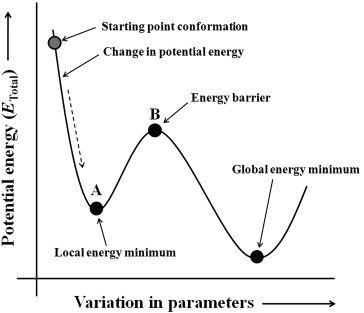
\includegraphics[scale=1]{images/energy-minimzation.jpg}
	\caption{Differenti fasi energetiche di una molecola durante la sua minimizzazione energetica. Fonte\cite{ROY2015151}}
	\label{fig:energy-minimization}
\end{figure}

\subsubsection{Molecular dynamics}

È possibile spingere l'algoritmo di minimizzazione energetica fuori da punti di minimo locale fornendo energia extra, ad esempio innalzando la temperatura del sistema (ovvero aggiungendo calore virtuale). L'energia aggiunta consente agli atomi del sistema di incrementare i loro movimenti e nuove configurazioni fuori dalle barriere energetiche vengono create. Questo metodo è chiamato \textit{Molecular dynamics} (MD) e si focalizza sui movimenti dipendenti dal tempo degli atomi nel sistema. I calcoli sono realizzati in accordo alla meccanica classica. 

\par Agli atomi viene assegnata una velocità iniziale (proporzionale alla temperatura) e continuano a muoversi nello spazio secondo i corrispondenti cambiamenti nell'energia potenziale del sistema. Il movimento di ogni atomo nel sistema è calcolato in base alla sua energia in quel dato momento.

\par Le simulazione di MD sono eseguite in cicli ripetitivi di \textit{riscaldamento} e \textit{raffreddamento} (metodo conosciuto nel mondo informatico come \textit{simulated annealing}, in riferimento al processo di tempra dei metalli). Nella fase di riscaldamento vengono superate le barriere energetiche mentre la fase di raffreddamento (seguita dall'\textit{energy minimization}) consente al sistema di rilassarsi in configurazioni con minor energia.

\par Un metodo comune per rendere la ricerca con MD più efficiente è di spezzarla in due fasi:
\begin{itemize}
	\item ricerca a bassa risoluzione per trovare una collezione di strutture con interazioni non polari (basato sulla nozione che il nucleo delle proteine globulari sia idrofobico)
	\item ricerca ad alta risoluzione fra le strutture selezionate nel primo step
\end{itemize}

\subsubsection{Limiti dell'approccio fisico e parziali soluzioni}
Sebbene simulare il ripiegamento proteico seguendo la meccanica classica possa apparire un approccio attraente, questo è pratico solo per piccole proteine e usando alte risorse computazionali: lo spazio di ricerca è enorme e il problema è computazionalmente intrattabile in modo deterministico (è NP-hard)\supercite{abbass2020enhancing}.

\par I metodi di MM/MD trovano difficilmente impiego in processi biologici rilevanti come il protein folding. Alcuni problemi riguardano l'approssimazione in sé del campo di forza, la sua accuratezza e i possibili doppi conteggi delle forze in gioco (es. interazioni ioniche e legami idrogeno calcolate in due espressioni differenti). 

\par Un altro problema, sempre nell'approssimazione dell'energia libera con campi di forza, è che forniscono sì l'energia potenziale ma non l'entropia. L'unico modo per stimare l'entropia e l'energia libera dai calcoli per l'energia potenziale è eseguire questi calcoli su tutte le possibili configurazioni del sistema e poi integrarli. Il problema risiede quindi nell'impossibilità di compiere la totalità di questi calcoli a causa delle rappresentazioni esplicite usate nelle simulazioni di MD. In particolare è difficile considerare tutte le configurazioni del solvente acquoso. Ciò che si sta calcolando non è l'energia libera ma un \textit{potenziale di forze medie} (PMF). In conclusione le simulazioni di MD non sono consigliate per descrivere gli effetti dei solventi.

\subsubsection{Mean field approach}
Per ovviare parzialmente al problema delle rappresentazioni esplicite è possibile descrivere \textit{implicitamente} parti del sistema che vengono descritte da una proprietà media, per questa ragione tale approccio è chiamato \textit{mean field}. Un esempio è la descrizione del solvente, la parte "meno" interessante in genere, come una massa omogenea descritta dalla sua \textit{dielettricità} \footnote{proprietà di un mezzo non conduttore di essere sede di un campo elettrostatico}, conosciuto anche come approccio \textit{continuum-solvent}, vedi fig. \ref{fig:mean-field}.

\begin{figure}[!htb]
	\centering
	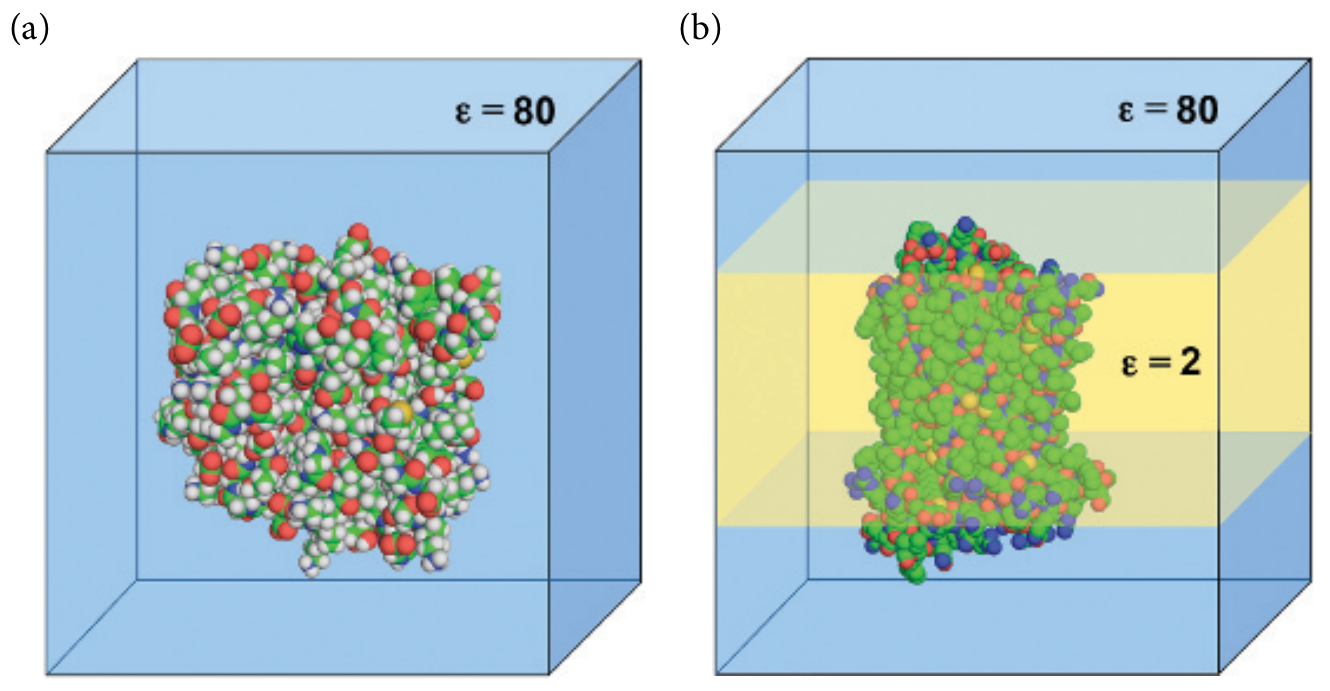
\includegraphics[scale=0.4]{images/mean-field.png}
	\caption{Descrizione con approccio mean-field di un sistema, il solvente è descritto implicitamente mentre la proteina esplicitamente. $\epsilon$ indica la dielettricità. (A) proteina in un solvente acquoso altamente dielettrico. (B) proteina di membrana in un ambiente eterogeneo. Il solvente acquoso è altamente dielettrico mentre la lastra semi-trasparente gialla, che rappresenta la regione biologica di doppio strato lipidico, è poco dielettrica. Fonte\cite{kessel_ben-tal_2018}}
	\label{fig:mean-field}
\end{figure}

Ovviamente, essendo una forte approssimazione, alcuni aspetti del sistema reale sono ignorati, come le interazioni fra gli atomi delle proteine e le molecole d'acqua. Tale problema si esacerba quando il solvente è una membrana. \\

\par Un altro compromesso è l'approccio \textit{mixed force fields} che combina calcoli espliciti sulla proteina e calcoli impliciti sul solvente. Viene usata l'equazione di Poisson-Boltzman (PBE) per calcolare accuratamente l'energia libera elettrostatica, legando così l'effetto polarizzante delle cariche con il loro ambiente. Essendo però un calcolo oneroso viene in genere risolta l'equazione generalizzata di Born (GB). A partire da queste due equazioni, che calcolano la componente elettrostatica dell'energia libera, è possibile calcolare l'intera \textit{free energy}, in modo abbastanza accurato, con calcoli che si rifanno alla surface area (SA, vedi parte finale della sez. \ref{sec:termodinamica-forze-idrofobiche}). 

\par Questi metodi sono chiamati \textit{PBSA} e \textit{GBSA} rispettivamente, e come si è visto permettono un calcolo più preciso dell'energia libera. Questi possono a loro volta essere combinati con la MM per rappresentare anche le interazioni del sistema (\textit{MM-PBSA, MM-GBSA}) e sono oggi largamente utilizzati.

\par Un altro limite computazionale è il lasso temporale che si riesce a coprire. La maggior parte delle proteine si ripiega in microsecondi mentre le simulazioni riescono a coprire tempi che vanno dai pico ai nanosecondi. Grazie ad avanzamenti nelle risorse informatiche sono stati fatti dei passi avanti da questo punto di vista. Un caso interessante è \textit{Anton}, un supercomputer progettato specificatamente per ottimizzare simulazioni di MD capace di coprire 85$\mu s$ al giorno per un sistema molecolare di 23.000 atomi (180 volte più veloce di qualsiasi computer general-purpose). Altri progressi sono dovuti alla computazione parallela e alla computazione accelerata dalla GPU. Il calcolo distribuito (\textit{grid computing}), ovvero una larga rete di computer personali dedicati volontariamente al completamento di processi, ha permesso alla rete \textit{Folding@Home} (170.000 computer) di simulare l'intero processo di ripiegamento della proteina di legame dell'acetil coenzima A, composta da 86 residui e che richiede 10 millisecondi per ripiegarsi. Un'altra rete distribuita di calcolo è \textit{Rosetta@Home}, con 86.000 nodi e finalizzata al PSP. \\

\subsubsection{Conclusioni sull'approccio \textit{ab initio}}
I metodi \textit{ab initio} non sono attualmente in grado di predire la struttura della maggior parte delle proteine sulla sola base della loro sequenza. Ma sono molto abili nel farlo quando il punto di partenza della predizione è una struttura vicino a quella nativa. Questi metodi sono infatti ampiamente usati per raffinare le strutture grezze ottenute dalle determinazioni sperimentali (vedi sez. \ref{sec:experimentally-guided-prediction}). 

\par Il loro successo dipende ampiamente dall'accuratezza della funzione di energia, dall'efficienza dell'algoritmo di ricerca nello spazio conformazionale e dall'abilità di discernere strutture native da "esche" energeticamente intrappolate.
Nonostante le loro limitazioni i metodi \textit{ab initio} sono di grande interesse perché sono gli unici, in principio, derivare la vera struttura nativa delle proteine e possono quindi fornire intuizioni importanti per il protein folding problem. Hanno infatti fornito informazioni importanti sulla dinamica delle proteine e sono utilizzati anche nel \textit{protein engineering} e nel \textit{drug discovery}. 

}


\subsubsection{Valutazione \textit{knowledge-based}}
È anche possibile rimpiazzare il campo di forza con una funzione di valutazione \textit{knowledge-based}. Spesso queste funzioni sono composte di espressioni relative alla tendenza statistica di gruppi chimici, amminoacidi o atomi di interagire fra di loro. L'affidabilità della funzione di valutazione dipende dal database su cui si basa. 


\section{Manipolazione della sequenza di input}

\subsection{\textit{sequence alignment}} \label{sec:MSA}
- protein sequence alignment (poi MSA)
[Burkowski 6 p.167]
baxevanis 8 p.227


Certain software programs can display multiple sequences together to show the degree of similarity between them

This is called a sequence alignment and is commonly used to show the degree of relatedness between sequences

Le sequenze di proteine in genere risultano avere un grado di somiglianza maggiore rispetto alle sequenze nucleotidiche, questo è dovuto alla degenerazione del codice genetico e al fatto che quasi per ogni amminoacido esistono vari codoni che lo codificano, perciò differenti sequenze nucleotidiche possono codificare esattamente la stessa sequenze di amminoacidi.

\begin{figure}[!htb]
	\centering
	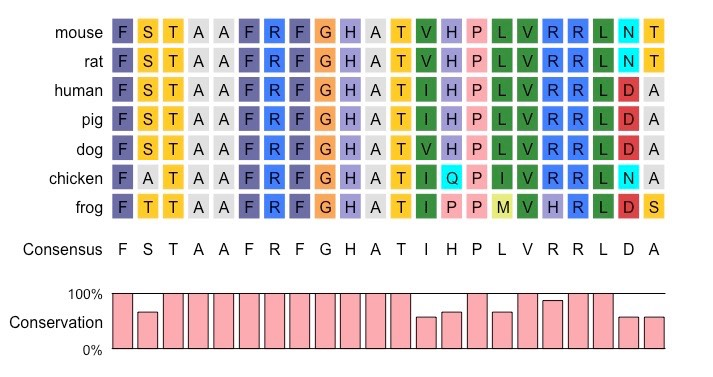
\includegraphics[scale=0.5]{images/msa.jpeg}
	\caption{Multiple sequence alignment schematica di una sequenza proteica di varie specie. Fonte\cite{msaBioNinja}}
	\label{fig:msa}
\end{figure}

\subsection{\textit{fold recognition}}
- praveen 2014
- pal 

Come si è già detto la struttura delle proteine è maggiormente conservata rispetto alle sequenze. Questo significa che proteine con differenti sequenze possono ancora formare strutture simili grazie a certe proprietà condivise codificate nelle loro sequenze. Se queste proprietà o ricorrenze statistiche potessero essere identificare, sarebbe possibile predire la struttura di una nuova proteina basandosi su un template che condivide le stesse proprietà, anche se loro sequenze sono diverse. Questa è l'idea su cui si basano i metodi di fold recognition. 
In altri termini, in questo approccio si cerca una proteina con struttura conosciuta (nel PDB) che abbia alcune proprietà nella sequenza o tendenze condivise con la proteina target: le due probabilmente hanno un ripiegamento simile o motivi strutturali simili.

\subsection{protein secondary structure prediction (PSSP)}
-wiki
-sejonwski 1989
-deOliveira 2021

\begin{figure}[!htb]
	\centering
	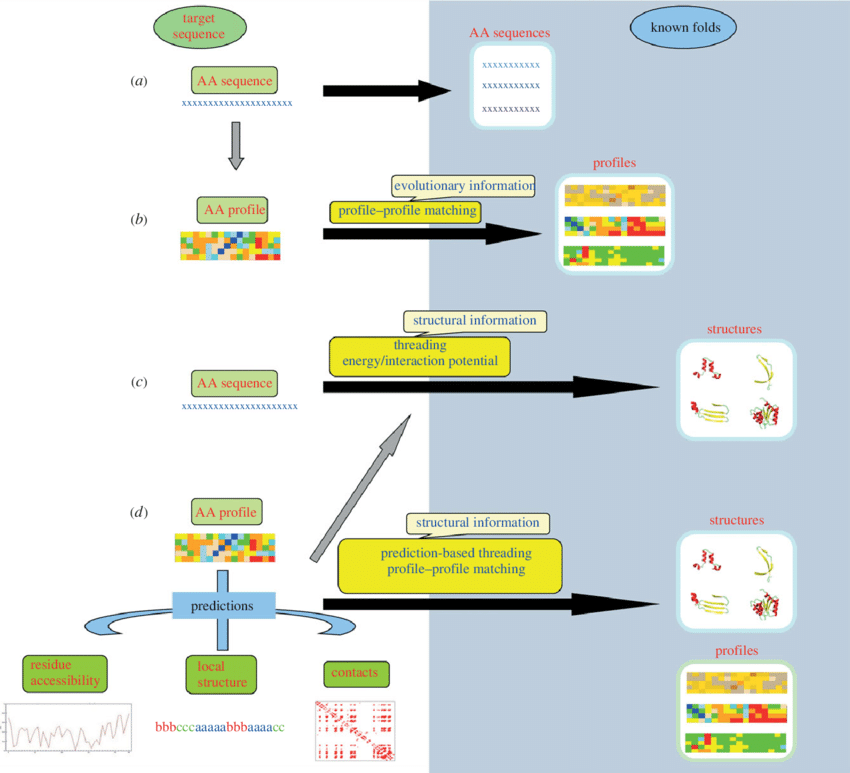
\includegraphics[scale=0.53]{images/threading-mappa.png}
	\caption{. Fonte\cite{joseph2014local}}
	\label{fig:fold-recognition}
\end{figure}

\subsection{\textit{contact prediction}}

\subsection{correlated mutation}

L'apparizione di mutazioni nelle sequenze delle proteine durante la loro evoluzione dipende da aspetti sia strutturali che funzionali. È interessante notare come l'analisi delle sequenze di famiglie di proteine mostri che certe posizioni tendono a \textit{coevolvere}. In altre parole l'apparizione di una mutazione in una posizione è accompagnata da una mutazione in un'altra posizione. 

\par È stato suggerito che un tale collegamento possa avvenire in posizioni vicine nello spazio tridimensionale e che i residui considerati interagiscano fra loro. Se una mutazione in una posizione porta a una distruzione della sua interazione con la posizione adiacente, una mutazione compensatoria di quest'ultima potrebbe rimediare al problema.

\par Ad esempio, se due posizioni erano originariamente polari e coinvolte in un'interazione elettrostatica favorevole, la mutazione di una posizione da polare a non polare distruggerebbe l'interazione. Se però la posizione adiacente muta anch'essa da polare a non polare, l'interazione originale può tramutarsi in un'altra interazione favorevole, stavolta non polare.

\par Ciò suggerisce che sia possibile inferire posizioni a contatto nella struttura ripiegata di una proteina analizzandone le variazioni nella sequenza attraverso la sua evoluzione e osservando quali posizioni sono \textit{coevolute}. Gli accoppiamenti evoluzionisticamente inferiti possono essere usati come vincoli durante la modellazione.

\begin{figure}[!htb]
	\centering
	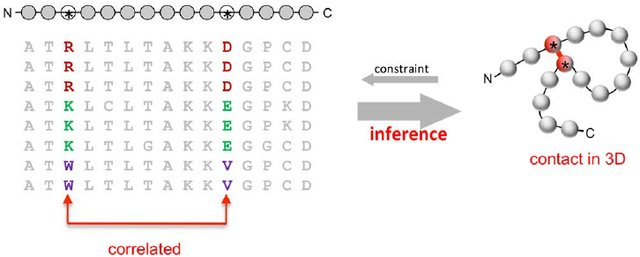
\includegraphics[scale=0.65]{images/correlated-mutation.jpg}
	\caption{In alto, sequenza della proteina da predire, in cui ogni amminoacido è un cerchio. Sotto, un MSA con le sequenze di una famiglia correlata, tutte con lo stesso ripiegamento. A destra l'inferenza del contatto delle posizioni coevolute. Fonte\cite{marks2011protein}}
	\label{fig:correlated-mutation}
\end{figure}

\par Ci sono 3 principali ostacoli a questo approccio: rumore statistico (molte correlazioni sono solo frutto di rumore e quindi insignificanti), correlazioni fra residui distanti e numero insufficiente di posizioni correlate. Il metodo non risulta applicabile quando ci sono poche sequenze omologhe. Nonostante l'idea non sia nuova, solo nell'ultimo decennio tali metodi sono divenuti abbastanza accurati da poter essere usati nel PSP; metodi noti sono EVfol, Rosetta-GREMLIN, FILM3, MetaPSICOV, ecc.



The hypothesis behind the approach was that if
mutations that occur at two positions in an MSA are
correlated, these positions are more likely to form a
contact in 3D space. This is because there is evolutionary
pressure to conserve the structures of proteins and a
mutation at one position may be rescued by a correspond-
ing mutation at a nearby residue. The accuracy of co-
evolution-based contact map prediction remained low for
many years due to the inability to distinguish between
direct and indirect interactions, where indirect interac-
tions occur when residues appear to co-evolve but do not
actually form contacts. For example, if Residues A and B
are both in contact with Residue C, A and B often appear
as if they co-evolve even when there is no physical
contact between them. There is evidence showing that
such co-evolution may have a functional cause [22] rather
than a structural one, which resulted in the failure of
structure-based contact derivation.\supercite{pearce2021deep}

Progress in contact prediction remained stagnant for some
time. However, a leap in contact prediction accuracy took
place when algorithms started utilizing global prediction
approaches. Early methods mainly predicted contacts
between residue pairs one-at-a-time using techniques
such as mutual information, thus ignoring the interactions
with other residue pairs and the global context in which
the interactions took place; this is largely why it was
difficult for these local methods to distinguish between
direct and indirect interactions. The introduction of
global statistical models determined through the use of
direct coupling analysis (DCA) was more successfully
able to distinguish between these direct and indirect
interactions [23,24]. 

Many DCA techniques fit a Markov random field (MRF),
or more specifically a Potts model, to an MSA. An MRF is


\section{Modellazione \textit{data-based} della struttura}

\subsection{\textit{homology modeling}}
{
	Nella modellazione per omologia ci si affida a somiglianze nella sequenza tra la proteina target e i template. I metodi per omologia sono perciò basati sul paradigma: \\
	\say{\textit{la sequenza codifica per la struttura}}.
	
	\par Sono metodi basati anche sull'osservazione che la struttura terziaria è più conservata della sequenza amminoacidica. Di conseguenza ci si aspetta una significativa somiglianza nella struttura fra proteine che condividono una notevole somiglianza tra le sequenze, anche non totale.
	
	\par In altri termini, due sequenze amminoacidiche molto simili (\textit{omologhe}) , in due proteine differenti ma evoluzionisticamente collegate, dovrebbero acquisire la stessa struttura locale.
	
	\par Un approccio che utilizzi la modellazione per omologia consiste tipicamente nei seguenti passi:
	\begin{enumerate}
		\item ricerca e selezione del template
		\item costruire un MSA (Multiple Sequence Alignment) che includa la proteina target e i template
		\item assegnare le coordinate spaziali dei template alla sequenza della proteina target
		\item raffinamento della struttura modello
		\item valutazione e validazione della struttura risultante
	\end{enumerate}
	
	\begin{figure}[!htb]
		\minipage{0.48\textwidth}
		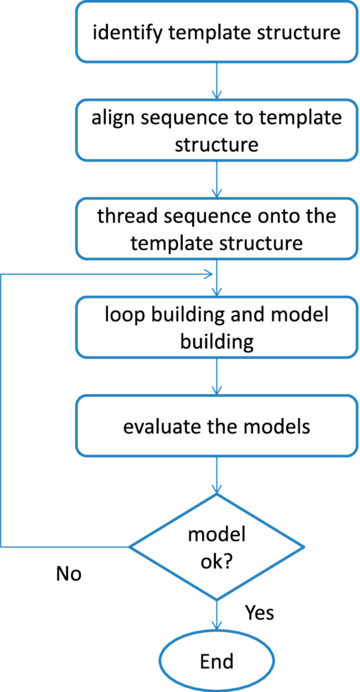
\includegraphics[scale=0.43]{images/homology1.png}
		\caption{Diagramma di flusso della modellazione per omologia. Fonte: \cite{sliwoski2014computational}}
		\label{fig:omologia-flusso}
		\endminipage\hfill
		\minipage{0.48\textwidth}
		\centering
		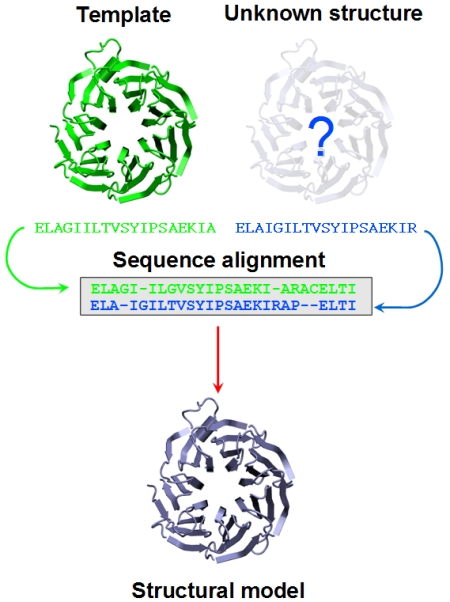
\includegraphics[scale=0.5]{images/homology2.jpg}
		\caption{Schema esemplificativo di una modellazione per omologia. Fonte \cite{UNIL-homology}}
		\label{fig:omologia-esempio}
		\endminipage\hfill
	\end{figure}
	
	Nel 1° step si cerca una struttura modello, almeno una, tra le strutture conosciute avente un'alta somiglianza di sequenza. È più semplice se la struttura di un una proteina omologa molto simile è stata già risolta. Ci sono però altri gruppi di proteine, come le proteine di membrana, le cui strutture risolte sono scarse. Trovare i giusti template e caratterizzare la loro omologia è ciò che determina in genere il successo dell'intera predizione (una somiglianza minore del 30\% avrà risultati molto scarsi, mentre sopra al 50\% la predizione ha buona probabilità di essere di buon livello). È possibile in ogni caso che vi sia una somiglianza \textit{locale} anche quando la somiglianza globale è scarsa. Le principali tecniche si dividono nelle seguenti categorie:
	\begin{itemize}
		\item pattern recognition e ricerche euristiche, ad esempio BLAST (Basic Local Alignment Search Tool) e FastA
		\item profile and iterative alignment methods, come PSI-BLAST e HMM (Hidden Markov Models), quest'ultimo molto usato
		\item structure based threading, come THREADER e FUGUE
	\end{itemize}
	
	\par Nel 2° step vengono sfruttate informazioni evoluzionistiche per migliorare l'allineamento tra le sequenze dei template e del target. È difficile stabilire allineamenti fra omologhi distanti, come nel caso di target \textit{eucarioti} e template \textit{procarioti}. La tecnica più usata oggi è l'MSA, altre tecniche usate sono: programmazione dinamica, MSA, threading, HMM ecc. Ci sono vari tool per creare MSA, ad esempio: Clustal$\Omega$, MAFFT, MUSCLE, T-Coffee. Possono venire utilizzati più MSA insieme per sopperire a problemi di disallineamento di piccole regioni. Il MSA viene illsutrato dopo la sezione \ref{sec:MSA}.
	
	\par Nel 3° step ad ogni segmento della sequenza target viene assegnato un insieme di coordinate spaziali in accordo ai risultati del MSA. Tool noti sono MODELLER (soddisfazione di vincoli spaziali), NEST, COMPOSER e SWISS-Model. La struttura ottenuta potrebbe essere però deformata a causa dell'utilizzo di più template e numerosi inserzioni e cancellazioni. Possono essere presenti lunghezze e angoli dei legami non ottimali e atomi sovrapposti.
	
	\par Per ovviare a tali problemi nello step 4 si applica un processo di raffinamento, specialmente per quanto riguarda i loop (\textit{loop modeling}, vedi sez. \ref{sec: loop-modeling}), regioni fodamentali per i siti di legame, e i residui (\textit{side chain modeling}). Vengono applicati algoritmi che confrontano caratteristiche geometriche ed effettuano calcoli energetici che identificano configurazioni atomiche sfavorevoli. 
	
	\par Nel 5° step si valuta l'affidabilità della predizione. Si dice che un modello è affidabile in generale quando è basato su un template corretto e un allineamento approssimativamente corretto. Si può valutare tale affidabilità in vari modi:
	
	\begin{itemize}
		\item alcune qualità della struttura costruita possono essere confrontate con delle tendenze statistiche 
		\item se ci sono vari modelli predetti si calcola l'energia libera e si sceglie la struttura con minor energia libera (ad es. tramite ProSa)
		\item stereochimica (relativa alle proprietà spaziali delle molecole), ad esempio con PROCHECK
		\item la conservazione evoluzionistica a livello amminoacidico può essere correlata con il loro stato "esposto" o "seppellito" (l'idea di partenza è che il nucleo della proteina rimanga inalterato e la superficie sia variabile), ad esempio Profiles3D
		\item se si hanno a disposizione dati sperimentali della struttura nativa della proteina si può validare il modello con la consistenza a essi.
	\end{itemize}
	
	\subsubsection{Efficienza e limiti}
	
	Con una somiglianza maggiore del 50\% si registra una RMSD tra 1 e 2 \angstrom, ma è importante notare che non sempre proteine omologhe (vicine sequenzialmente) condividono la stessa funzione e struttura. Un esempio sono le proteine del lievito Gal1 e Gal3: 73\% di identità e 92\% di somiglianza. Queste due proteine hanno però sviluppato differenti funzioni, con Gal1 che è una galattochinasi mentre Gal3 è un induttore trascrizionale\supercite{platt2000insertion}.
	
	\par Non c'è quindi una soglia che assicuri una sicura predizione della struttura: molte proteine con una lontana somiglianza possono svolgere la stessa funzione mentre altre altamente simili possono svolgere funzioni diverse. Una regola empirica è considerare sequenze con più del 30-40\% di somiglianza come sequenze con una struttura o funzione simile.
	
	\begin{figure}[!htb]
		\centering
		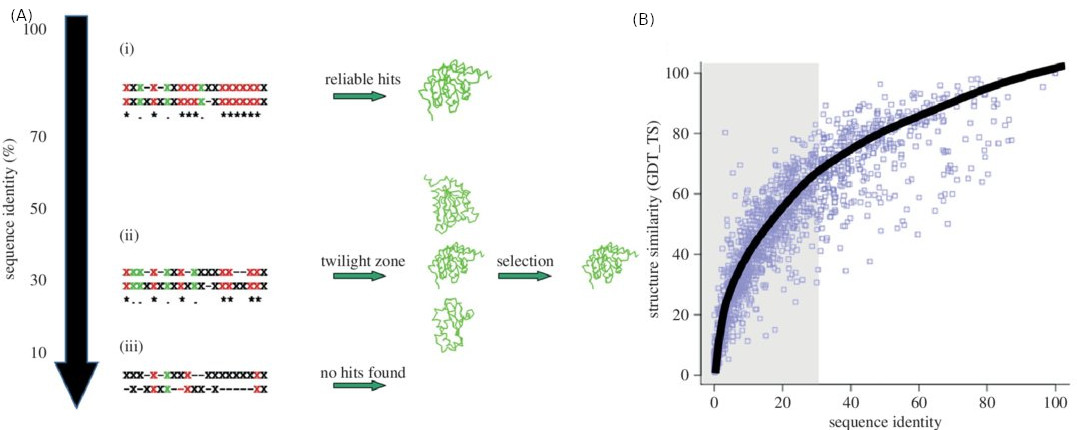
\includegraphics[scale=1.2]{images/homology-grafico.jpg}
		\caption{Risultati dei metodi per omologia alla variazione dell'identità nella sequenza. (A) Dimostrazione schematica dell'uso di confronti di sequenze per identificare omologie strutturali. 'X' indica un qualsiasi amminoacido. (i) identità > 70\%: semplici allineamenti di sequenza sono sufficienti per trovare il corretto ripiegamento. (ii) Tra il 20 e il 30\% non sempre è possibile trovare il corretto ripiegamento; è necessario effettuare ulteriori raffinamenti. (iii) a bassi livelli l'utilità di questo metodo è molto bassa. (B) Somiglianza strutturale (in GDT\_TS score) al variare dell'identità della sequenza. Anche al 30\% il livello di somiglianza è significativo. Fonte\cite{joseph2014local}}
		\label{fig:omologia-grafico}
	\end{figure}
	
	\par Un'osservazione fondamentale risiede sulle basi in sé del metodo: dato l'affidamento pressoché totale nella modellazione comparativa, la struttura modello è condizionata necessariamente a essere più simile ai template che alla reale struttura nativa della sequenza target, nonostante i vari processi successivi di raffinamento che, data la loro natura approssimativa, non sono perfetti. 
	
	\par I problemi maggiori risultano nelle regioni con bassa somiglianza, come ci si può aspettare. Si sta parlando specialmente dei \textit{loop}, soggetti a mutazioni considerevoli durante l'evoluzione.
	
	\par Si incorrono in problemi con la modellazione per omologia quando si trattano proteine che non hanno omologhe tra le strutture conosciute, come le proteine di membrana, le quali sono difficili da da cristallizzare. \\
	
	\subsubsection{Conclusioni sulla \textit{modellazione per omologia}}
	
	\par Nonostante tutte le osservazioni fatte, \textit{la modellazione per omologia è correntemente il miglior metodo computazionale per predire la struttura delle proteine} e la sua applicabilità è destinata a crescere con l'aggiunta di nuove strutture determinate sperimentalmente da poter essere usate come template.
	
	\par La sfida principale che questi metodi hanno affrontato, e che AlphaFold ha "vinto", era raggiungere almeno una RMSD di 3\angstrom. Le sfide ancora da superare riguardano l'accuratezza su grandi proteine, su proteine con un contenuto significativo di strutture $\beta$ e la modellazione di proteine multi-dominio e di membrana.
	
	\par Oltre alla PSP i metodi per omologia sono anche usati nel drug design (per studiare le differenze strutturali fra le proteine bersagliate dallo stesso farmaco) e nello studio dei meccanismi catalitici.
	
}

\subsection{\textit{threading modeling}}

\subsection{\textit{fragment-based modeling}}
-abbass 

\par Un possibile metodo di azione è la \textit{frammentazione delle proteine}, nel quale i calcoli sono realizzati su piccoli frammenti della proteina e poi integrati. Un esempio è il software QUARK. L'approccio \textit{fragment-based} è usato nei metodi che combinano predizioni \textit{template-based} con assemblaggi \textit{ab initio}.

-- parla dell'assemblaggio dei frammenti. È ab initio?

\subsection{\textit{loop modeling}} \label{sec: loop-modeling}
{
I loop sono regioni della struttura proteica con ruoli spesso cruciali (interazioni con altre proteine, siti di legame con molecole ecc.). Allo stesso tempo sono molto variabili nella loro sequenza e struttura rispetto alle altre regioni. Si trovano generalmente sulla superficie delle proteine e le loro strutture sono note per essere difficili da predire.

\begin{figure}[!htb]
	\minipage{0.48\textwidth}
	\centering
	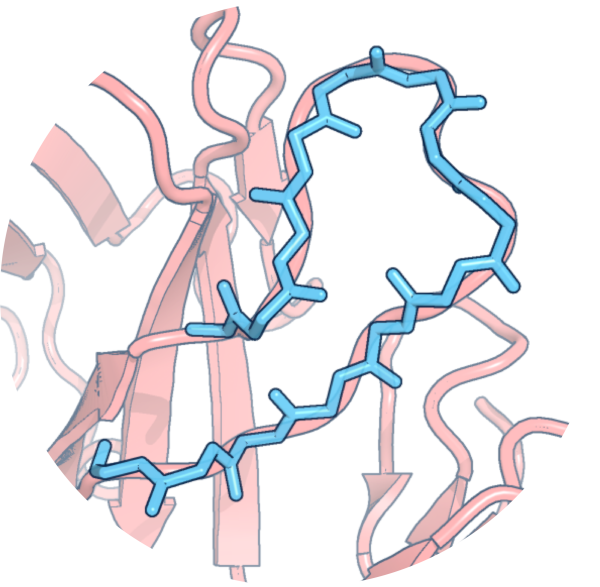
\includegraphics[scale= 1]{images/fread.png}
	\caption{Disegno di un loop in celeste. Fonte \cite{FREAD}}
	\label{fig:loop-example}
	\endminipage\hfill
	\minipage{0.5\textwidth}
	\centering
	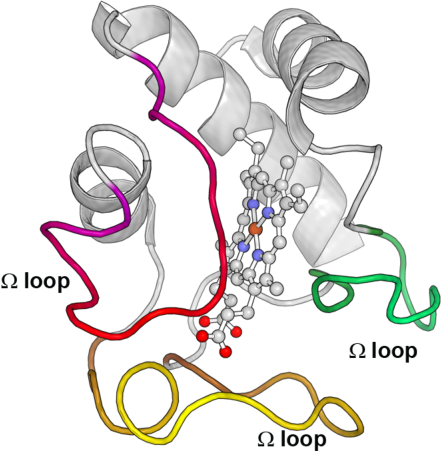
\includegraphics[scale=0.3]{images/loops.png}
	\caption{Omega loop. Sono spesso coinvolti nel riconoscimento molecolare e in funzioni regolatrici. Fonte: \cite{Papaleo2016TheRO}}
	\label{fig:omega-loops}
	\endminipage\hfill
\end{figure}

Il loop modeling non si applica solamente alla fase di raffinamento della modellazione per omologia della predizione di strutture proteiche. È importante anche nella predizione di frammenti mancanti nelle strutture determinate sperimentalmente. È stato stimato che in più della metà delle struttura depositate nel PDB ci siano segmenti mancanti, spesso loop\supercite{karami2018dareus}.

\par Problemi comuni nel loop modeling sono: decidere quale regione del modello sarà un loop; trovare il corretto allineamento di regioni di ancoraggio; la modellazione in sé del loop; le conformazioni di loop multipli, ecc.

\par Nella modellazione per omologia (nel PSP) si registrano spesso grandi deviazioni dai template omologhi: la modellazione dei loop rimane un problema aperto nella modellazione per omologia della struttura delle proteine\supercite{karamiLoop}. Le principali strategie per il loop modeling sono le stesse di quelle per la predizione dell'intera struttura:
\begin{itemize}
	\item \textit{data-based} (o knowledge-based), basati sull'assunzione di similarità sequenza-struttura, ovvero che loop con sequenze simili hanno anche conformazioni simili
	\item \textit{ab initio}, in cui viene esplorato lo spazio conformazionale
	\item approccio ibrido
\end{itemize}

\par Un protocollo comune per la modellazione, partendo da un modello della proteina senza loop e la sequenza del loop, è quello mostrato in figura \ref{fig:loop-modeling-approaches}, con i seguenti step:
\begin{itemize}
	\item generazione di tutti i possibili stati del loop (ab initio, data-based o ibrido)
	\item valutazione e raggruppamento
	\item raffinamento
\end{itemize}

\begin{figure}[!htb]
	\centering
	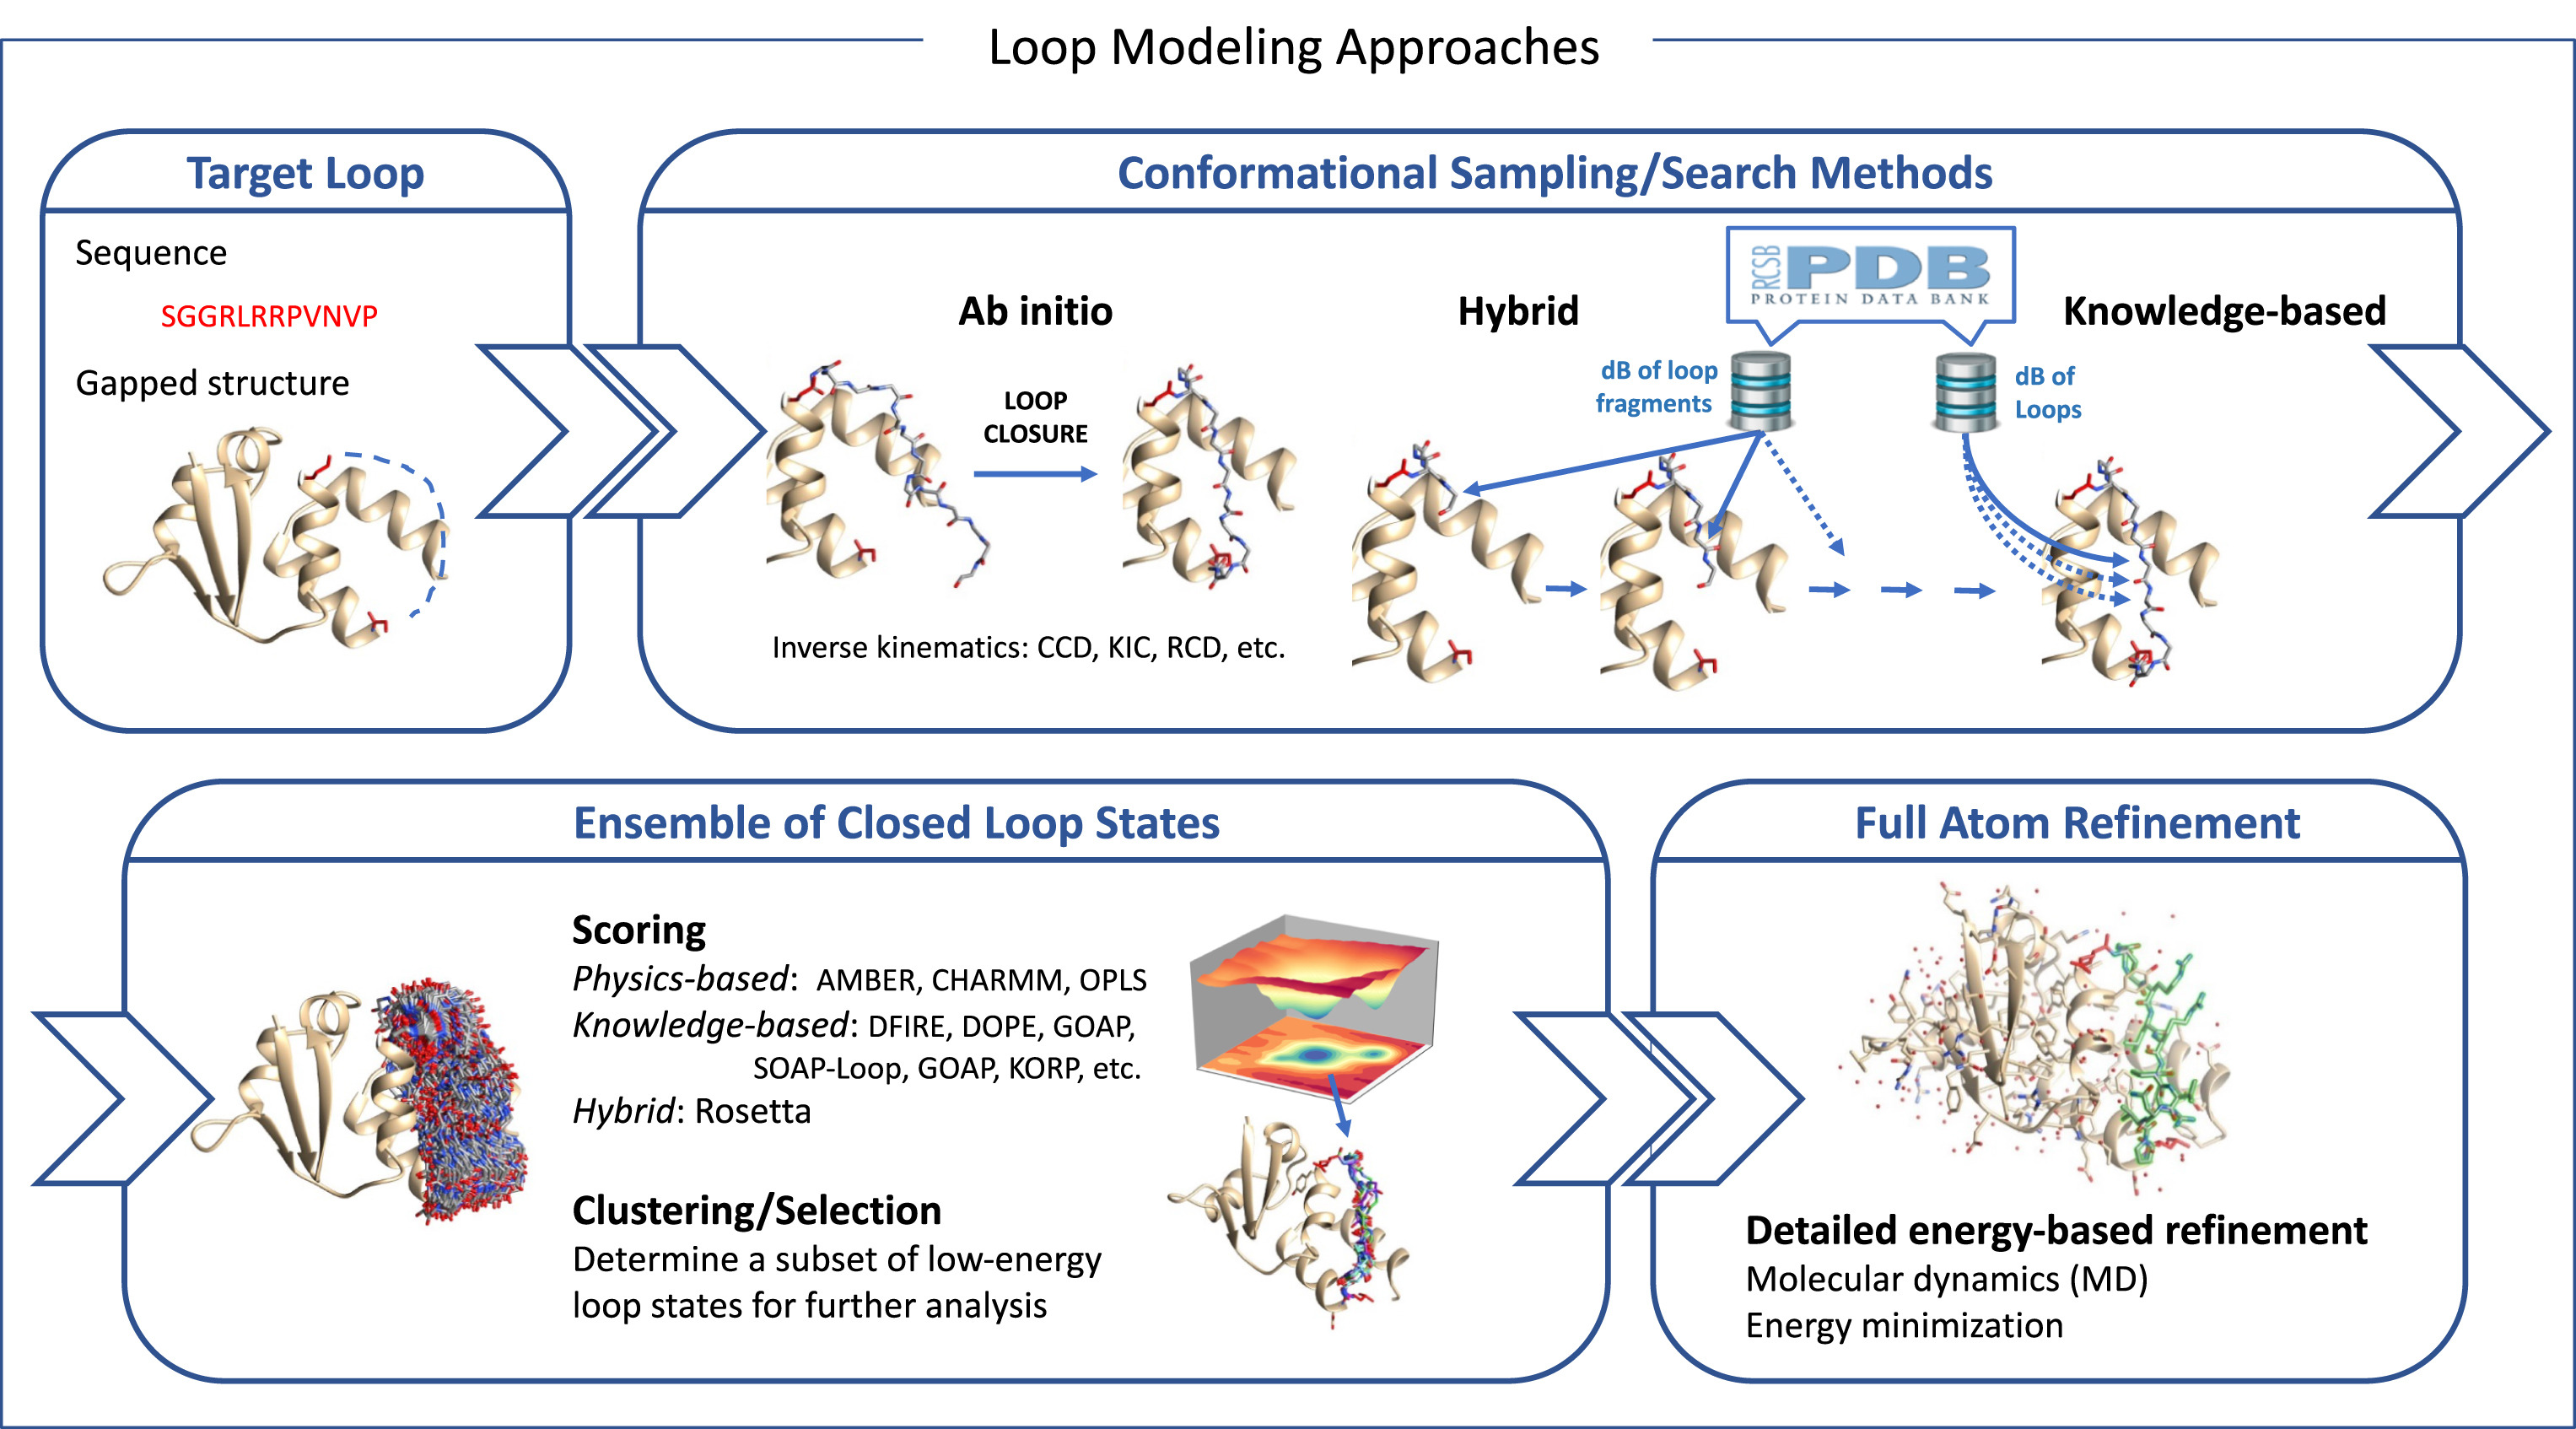
\includegraphics[scale=1]{images/loop-modeling-approaches.jpg}
	\caption{Approcci al loop modeling. Workflow schematico di un protocollo prototipo per la modellazione dei loop. Fonte\cite{barozet2021current}}
	\label{fig:loop-modeling-approaches}
\end{figure}

La ricerca su database è efficiente per famiglie specifiche ma i loop più lunghi di 4 residui devono essere comunque ottimizzati. I residui ai fianchi della regione del loop sono chiamati residui di \textit{ancoràggio} e sono utilizzati per effettuare la ricerca nei database. ArchPRED ad esempio considera le strutture secondarie ai fianchi del loop mancante, il loro orientamento relativo e il numero di residui mancanti per identificare conformazioni del loop candidate. È possibile usare una funzione di valutazione basata sull'energia per valutare la modellazione dei loop, ad esempio basata sulla stereochimica (come in CHARMM). 

\par Molti dei metodi raggiungono ottimi risultati per la predizione dei loop su strutture sperimentali in ambienti esatti (ovvero strutture cristallizzate a cui mancano le regioni dei loop). Ma nei modelli per omologia non si è ancora riusciti a raggiungere buoni risultati\supercite{karami2018dareus}. Metodi allo stato dell'arte sono in grade di predire conformazioni stabili di loop relativamente corti (fino a 12 residui)\supercite{barozet2021current}.
Seppur con le loro limitazioni, gli approcci correnti sono pronti per essere usati in problemi impegnativi come il loop design in enzimi e anticorpi.

\par I metodi \textit{ab initio} sono dipendenti dalle tecniche di ottimizzazione dell'energia e per questa ragione risultano essere lenti. Metodi \textit{ab initio} per il completamento della struttura cristallizzata allo stato dell'arte sono Rosetta-NGK e GalaxyLoop-PS2. CODA è un esempio di metodo ibrido che combina i due approcci nel loop modeling, così come Sphinx il quale prima esegue una ricerca data-based per trovare frammenti più corti del loop di interesse in modo da ottenere informazioni strutturali, successivamente applica metodi \textit{ab initio} per generare frammenti della corretta lunghezza. \\

\par Pochi metodi sono disponibili come web servers e quindi utilizzabili anche dai non esperti: GalaxyLoopPS2, LoopIng, Sphnix e DaReUS-Loop. Metodi locali sono invece MODELLER, Loopy, OSCAR-loop, Rosetta-NGK, LEAP e M-DISGro. Sono disponibili anche dei tool per la modellazione di loop specifici per gli anticorpi, come quelli offerti da SAbPred\footnote{Collezione di tool sviluppati da Oxford Protein Informatics Group (OPIG).}: Sphinx e FREAD (knowledge-based) che effettua una ricerca su database tenendo in considerazione i vincoli spaziali dei residui di ancoràggio.

\par Possono essere utilizzati anche simulazioni Monte Carlo e MD per investigare proprietà termodinamiche e cinetiche dei loop. Per quanto riguarda l'utilizzo di Deep Learning o Machine Learning per la modellazione dei loop, resta da dimostrare la capacità dei metodi ML/DL di generare modelli significativi di loop flessibili, nonostante in altre aree della bioinformatica strutturale si sia rivelato uno scenario con grande potenziale\supercite{barozet2021current}.

\par Uno dei metodi più recenti e con migliori risultati è DaReUS-Loop, un approccio  \textit{data-based} che identifica loop candidati estraendoli dal completo insieme delle strutture conosciute del PDB. Il filtraggio dei candidati si basa su confronti di conformazioni locali profilo-profilo insieme a una valutazione fisico-chimica. Applicato ai dataset del CASP11 e CASP12 mostra significativi progressi nell'accuratezza della predizione dei loop e propone una misura di confidenza che correla bene con l'accuratezza effettiva dei loop. I loro autori mostrano anche che oltre il 50\% dei modelli ben riusciti sono derivati da proteine non correlate: ciò suggerisce che frammenti di proteine, sotto simili vincoli, tendono ad adottare simili strutture (oltre la mera omologia)\supercite{karami2018dareus}. 

\begin{figure}[!htb]
	\centering
	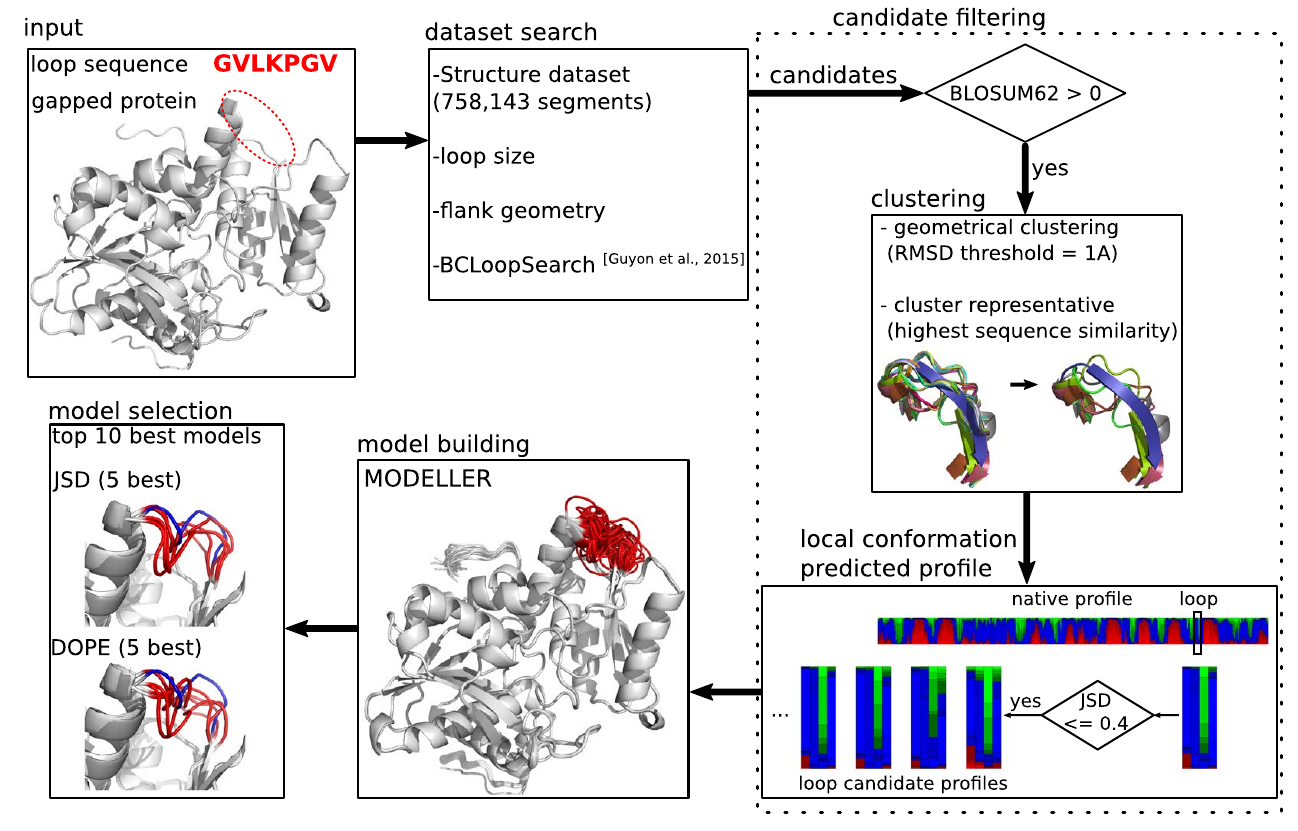
\includegraphics[scale=0.45]{images/dareus.png}
	\caption{DaReUS-Loop workflow. Da notare che dal 2019\supercite{karamiLoop} nel processo di costruzione del modello non è più usato MODELLER (non free) ma GROMACS. Fonte\cite{karami2018dareus}}
	\label{fig:dareus-workflow}
\end{figure}

I principali step del metodo sono mostrati in figura \ref{fig:dareus-workflow} e sono:
\begin{itemize}
	\item ricerca dei candidati del loop
	\item filtraggio dei candidati
	\item costruzione del modello
	\item model selection
\end{itemize}

Nell'ultimo step sono utilizzate 2 misure per valutare i modelli e vengono ritornati in output come predizioni finali i 5 migliori modelli per ogni metrica.

\begin{figure}[!htb]
	\centering
	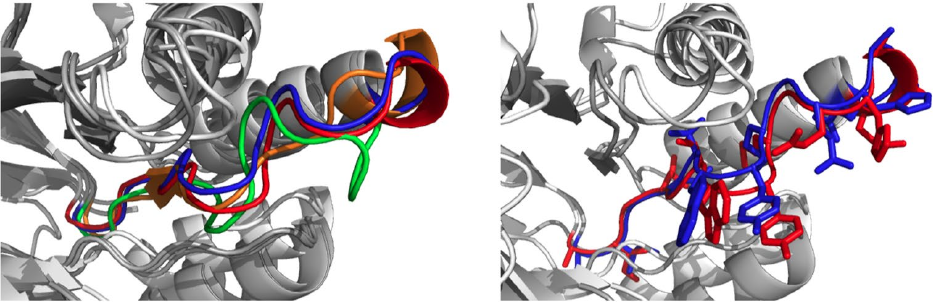
\includegraphics[scale=0.63]{images/dareus-confronto.png}
	\caption{Esempi di predizione di un loop lungo (15 residui) della proteina target T0807 del CASP11 a confronto. Blu=DaReUS-Loop, verde=Rosetta NGK, arancione=GalaxyLoop-PS2, rosso=struttura cristallizzata. La RMSD di ogni loop predetto rispetto al loop nativo è riportata di seguito. DaReUS-Loop: 1.3\angstrom, NGK: 3\angstrom, PS2: 2.9\angstrom. Nella colonna a destra sono riportate le catene laterali della struttura nativa e di quella predetta da DaReUS-Loop. Fonte\cite{karami2018dareus}}
	\label{fig:}
\end{figure}

}

\section{Case Study: \textit{TASSER}}
-tasser papers
-kessel
-abbass
-pearce 2021


\section{Determinazione sperimentale delle strutture} \label{sec:experimentally-guided-prediction}

La determinazione sperimentale della struttura delle proteine ha vissuto dei progressi significativi col passare degli anni ed è di grande importanza per i metodi computazionali di PSP.


- come le proteine sono studiate [alberts, 4.4 p.158]
- metodi sperimentali 
alberts p.168
pal 6 p.126 ma è molto tecnico
wiki-protein folding, 
baxevanis 12 p.363

• storia dei metodi sperimentali (Pal) \\
• cristallografia a raggi-x \\
• NMR, risonanza magnetica nucleare \\
• Cryo-EM (electron microscopy) \\



\section{Storia della comprensione delle proteine}
- alberts p.160
- psp-wiki
- levitt 2001, birth of structural biology \\ \\


L'approccio \textit{ab initio} è emerso negli anni '60 a partire dal campo della chimica computazionale. Nel 2013 il premio Nobel per la chimica è stato assegnato proprio a quegli scienziati che hanno contribuito sin da quegli anni al campo della biofisica molecolare computazionale (Warshel, Levitt, Karplus).

\par Le predizioni di strutture basate sui metodi \textit{ab initio} sono emerse nella metà degli anni '80, prima per piccoli peptidi e poi per polipeptidi. Il primo programma per calcolare l'energia potenziale nelle proteine è stato sviluppato nel 1969 da Lifson e Levitt\supercite{levitt1969refinement}.

\par La prima simulazione di MD su una proteina è stata realizzata nel 1977 da McCammon, Gelin e Karplus\supercite{mccammon1977dynamics}, studiando la dinamica di ripiegamento di una proteina di 58 amminoacidi rappresentata esplicitamente ma simulata nel vuoto. Questo studio seguì il lavoro pionieristico di Levitt e Warshel del 1975 (\textit{Computer simulation of protein folding}\supercite{levitt1975computer}) sulla stessa proteina che era però rappresentata in modo più semplicistico: ogni amminoacido era rappresentato da due sfere. 

\subsubsection{anni '90, database, omologia, progetto genoma}

Around the beginning of the 1990s, a new field in biology called ‘bioin-
formatics’ emerged, in which scientists sought to predict the characteristics of new pro-
teins on the basis of properties of their sequences

\subsubsection{CASP e AlphaFold}

A test of homology modeling efficiency carried out in 2007 has
shown that in single-domain proteins comprising 90 residues or fewer, the structures pre-
dicted by this method differed from their corresponding native structures by 2 to 6 \supercite{dill2008protein}.



Interestingly, in the first rounds of CASP, secondary structure prediction was a separate category. This
category was cancelled after the organizers noticed that the winners in this category used a somewhat circular
approach. They predicted the 3D structure and used their model structure to decipher the secondary structure
elements.

\clearpage